\section{Methods}
We create cell-type specific connectivity matrices using a model trained on murine viral-tracing experiments.
This model predicts projection patterns of different neuron classes at different locations within the brain that are more accurate than simple averages over nearby experiments in cross-validation.
This section describes the data used to generate the model, the model itself, the evaluation of the model, and the use of the model in creation of the connectivity matrices.
We then give exploratory analyses of the resulting connectivities that illustrate their key features. 
Additional information on our methods is given in Supplemental Section \ref{sec:supp_methods}.
\newpage
\begin{figure}[H]
\subfloat[]{
\label{fig:mouse}
    
\includegraphics[width=0.3\textwidth]{figs/figure1a.png}}
\subfloat[]{
\label{fig:injproj}
    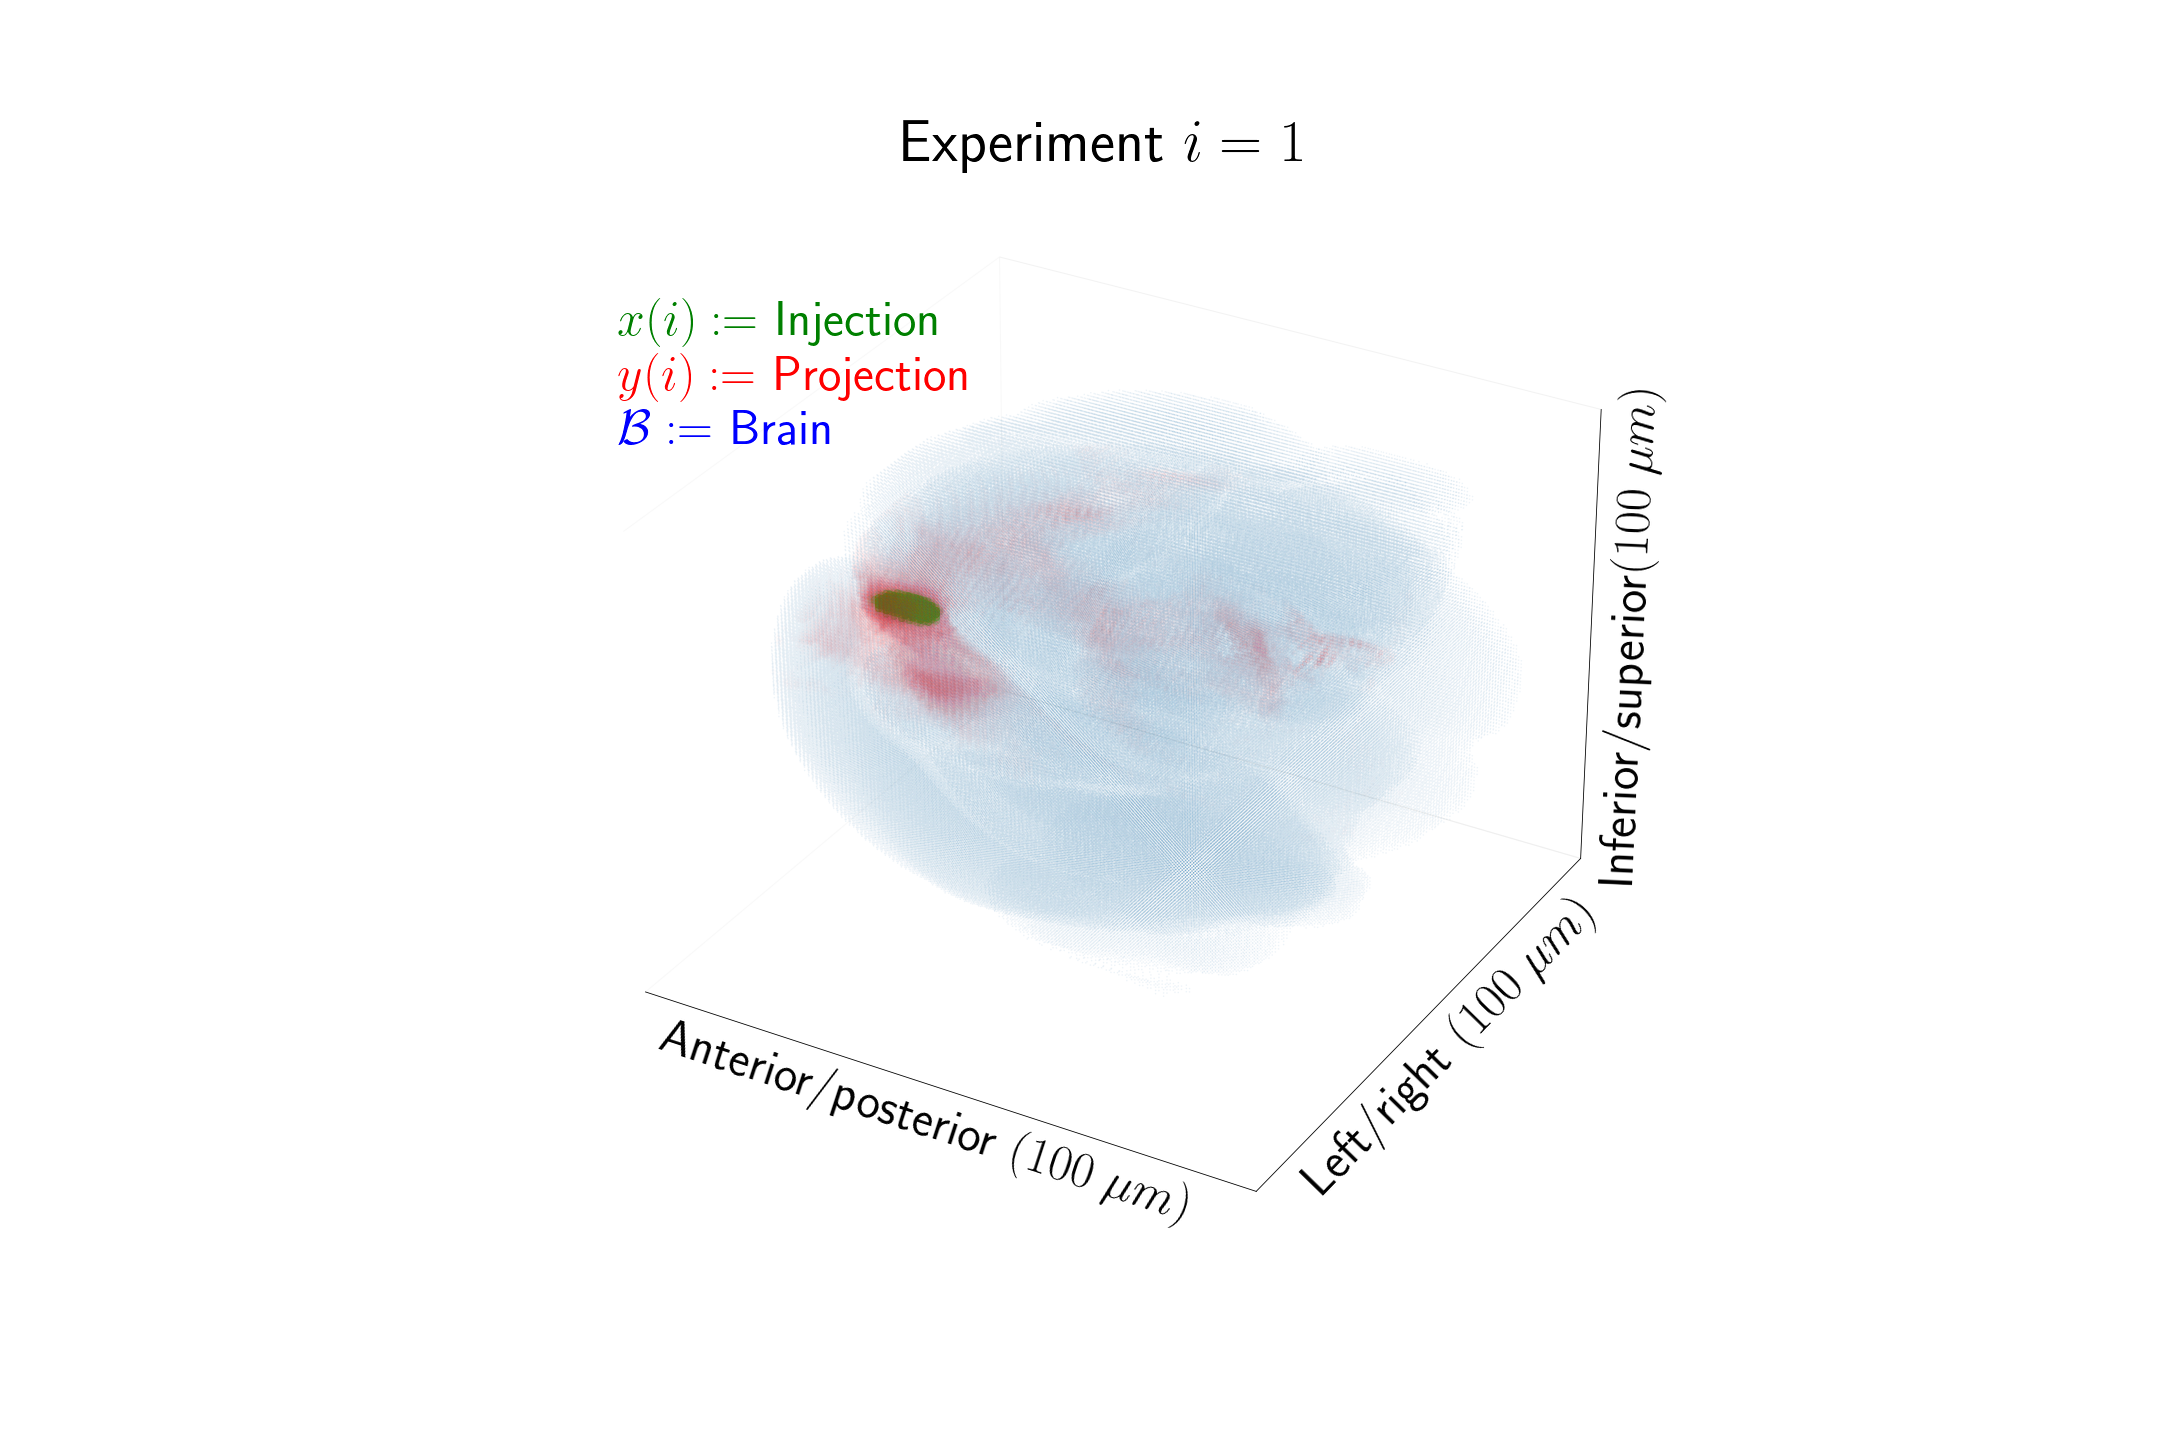
\includegraphics[width=0.4\textwidth]{figs/inj_proj_figure_v2.png}}
\subfloat[]{
\label{fig:segment}
    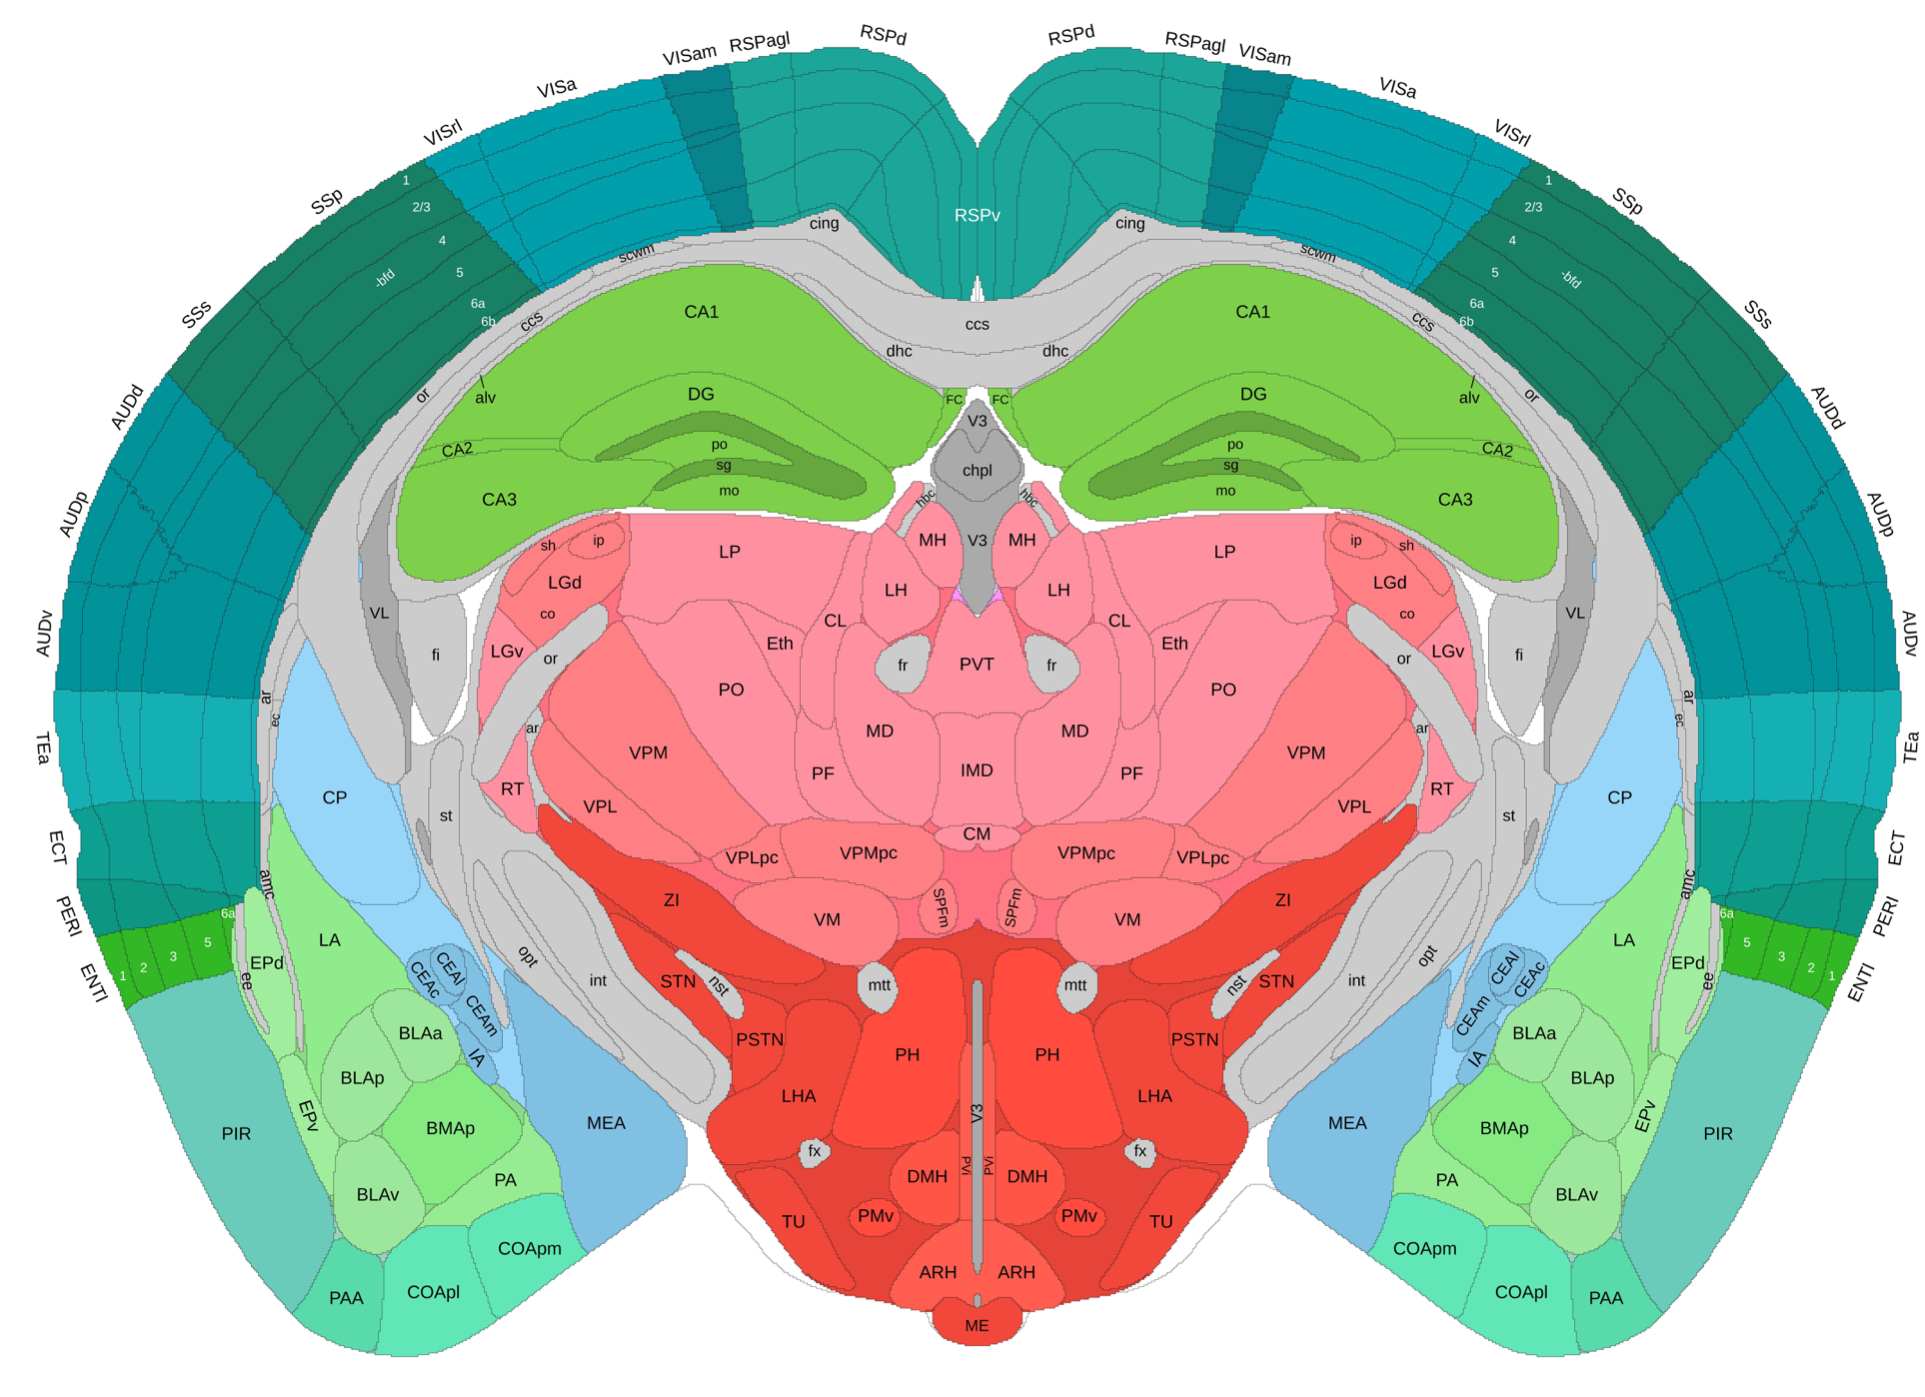
\includegraphics[width=0.3\textwidth]{figs/fig1c.png}}
    \newline
 \subfloat[]{
 \label{fig:ontology}
    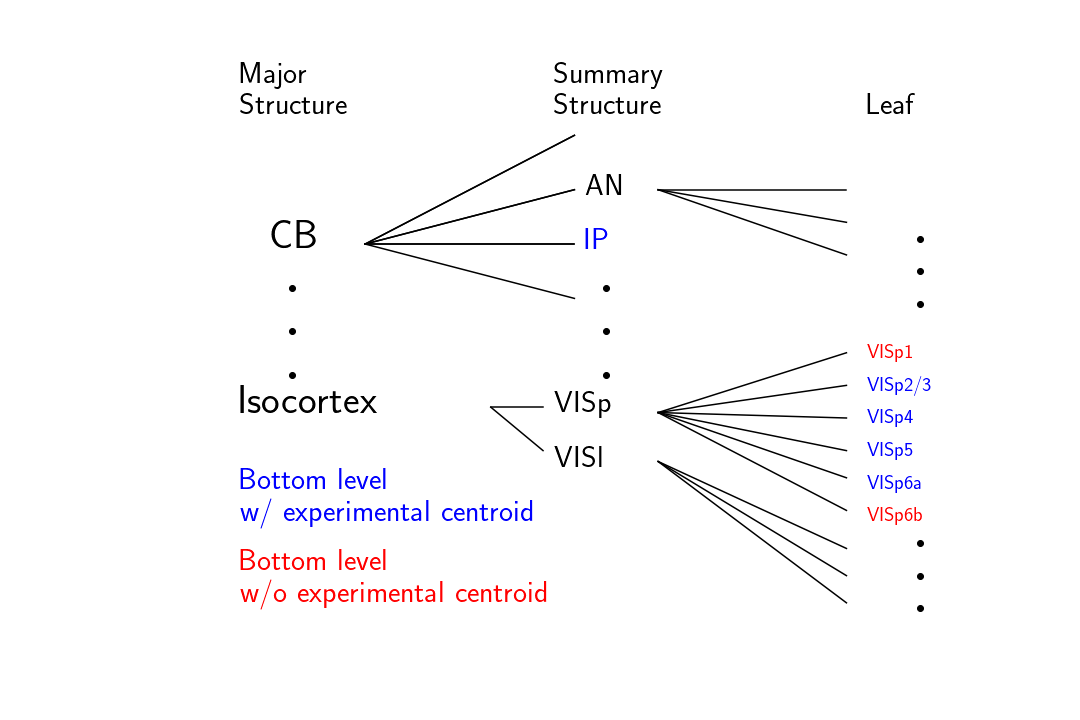
\includegraphics[width=0.35\textwidth]{figs/figsforpres/ontologyfigure.png}}
\subfloat[]{
 \label{fig:top}
    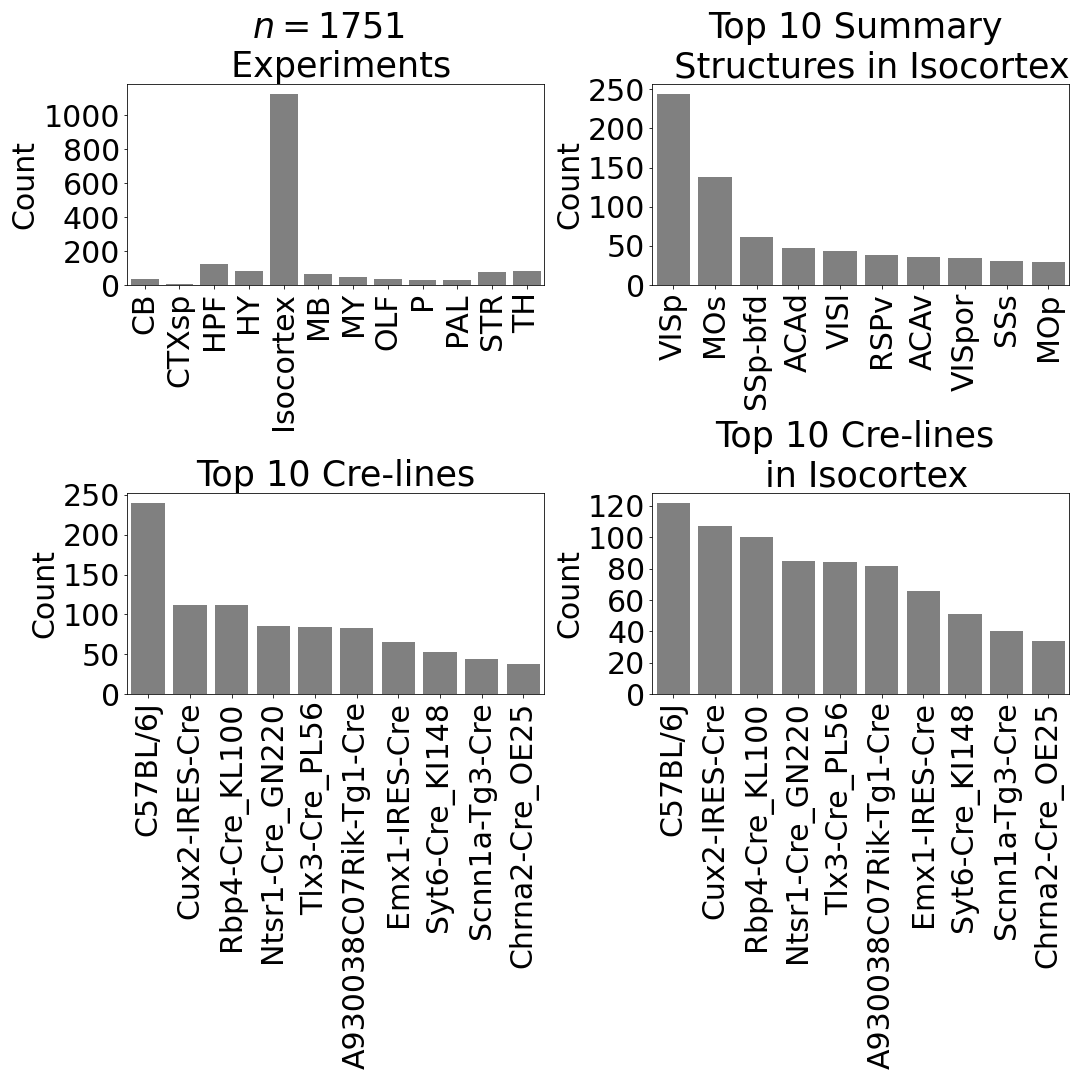
\includegraphics[width=0.35\textwidth]{figs/figsforpres/datasummary.png}}
\subfloat[]{
 \label{fig:combos}
    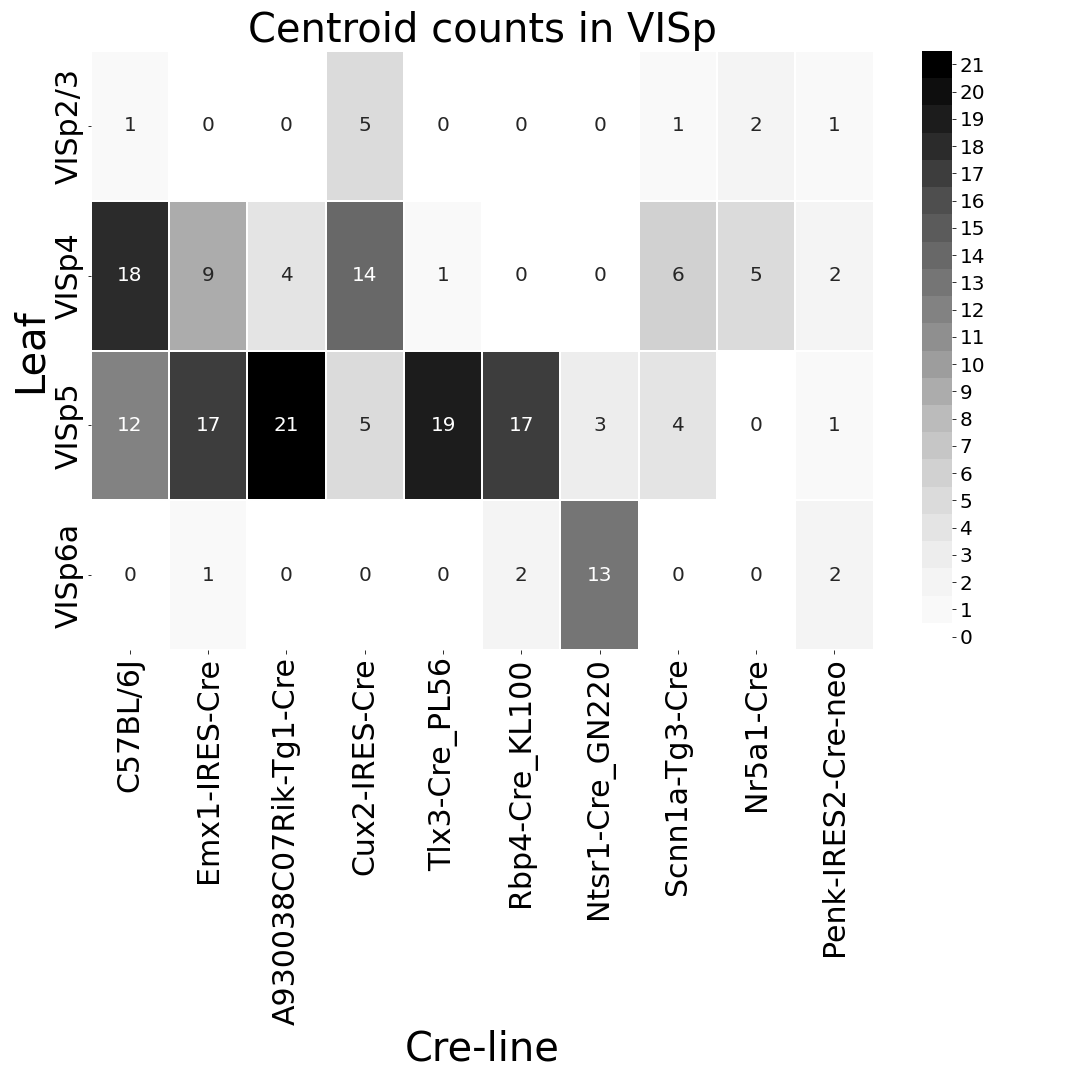
\includegraphics[width=0.35\textwidth]{figs/figsforpres/visp_counts.png}}   
    \caption{Experimental setting.  a) Within the brain (blue), injection (green) and projection (red) areas are determined via histological analysis and alignment to the Allen Common Coordinate Framework (CCF). b) An example of the segmentation of projection and injection for a single experiment. \label{fig:1b} c) Example of structural segmentation within a horizontal plane. d) Explanation of nested structural ontology highlighting lowest-level and data-relevant structures. e) Abundances of crelines and structural injections. f) Cooccurence of layer-specific centroids and creline within VISp}
    \label{fig:data}
\end{figure}

\newpage
\subsection{Mice}

\skcomment{Experiments involving mice were approved by the Institutional Animal Care and Use Committees of the Allen Institute for Brain Science in accordance with NIH guidelines.}

\subsection{Data}

Our dataset $\mathcal D$ consists of $n=1751$ experiments from the Allen Mouse Connectivity Atlas.
Figures \ref{fig:mouse} summarizes the multistage experimental process used to generate this data.
In each experiment, a GFP-labelled transgene casette with a potentially cre-specific promoter is injected into a particular location in a cre-driver mouse.
This causes fluorescence thats depends on the localization of cre-recombinase expression within the mouse.
While frequently this localization corresponds to a specific cell-type, it can also correspond to a combination of cell-types.
For example, in wild-type mice injected with non-cre specific promoters, fluorescence is observed in all areas projected to from the injection site, regardless of cell-type.
Thus, we use the term \textit{neuron class} to describe the neurons targeted by a specific combination of transgene and mouse-line.
This is the notion of cell-type specificity that we model.

After injection, the resultant fluorescent signal is imaged, and aligned into the Allen Common Coordinate Framework (CCF) v3, a three-dimensional idealized model of the brain that is consistent between animals.
This imaging and alignment procedure (described in detail in \citep{Harris2019-mr}) records fluourescent intensity discretized at the $100 \; \mu$m \textit{voxel} level. 
The image is histologically segmented into \textit{injection} and \textit{projection} areas corresponding to areas of transduction and transduction/transfection, respectively.
An example for a single experiment is given in Figure \ref{fig:injproj}.

Our goal is the estimation of {\textit structural connectivity} from one structure to another.
Thus, a visual depiction of this structural regionalization for a slice of the brain is given in Figure \ref{fig:segment}.
For different areas of the brain, the Allen Atlas contains different depths of discretization.
We denote these levels as Major Structures, Summary Structures, and Leafs.
As indicated in Figure \ref{fig:ontology}, the dataset used to generate the connectivity model reported in this paper contains certain combinations of structure and neuron class $(S,V)$ frequently, and others not at all.
A summary of the most frequently assayed neuron classes and structures is given in Figures \ref{fig:top} and \ref{fig:combos}.
Since users of the connectivity matrices may be interested in particular combinations, or interested in the amount of data used to generate a particular connectivity estimate, we exhaustively present this information about all experiments in Appendix \ref*{supp_sec:data}.

We can preprocess this publically available data in several ways.
A detailed mathematical description of these is given Appendix \ref{sec:dp}.
%We represent fluorescences as arrays $\mathcal F= \mathcal B \times \mathbb R^+$, where $B \subset [1:132] \times [1:80] \times [1:104]$ corresponds to the subset of the voxelized $(1.32 \times 0.8 \times 1.04)$ cm rectangular space occupied by the standard mouse brain.
%We also normalize projections by total intensity to account for differences in the cre-driven expression of eGFP via the various transgene promoters.
%For a given experiment, we denote injection and projection tensors as $x(i) \in  \mathbb R^B$ and $y(i)\in  \mathbb R^B$, respectively.
%We also have access to a regionalization map as $r: \mathcal B  \to \mathcal R $ which induces a map of connectivities $r_*: \mathcal F \to \mathcal R \times \mathbb R^+$.
%Given a vector $a \in \mathbb R^p$, we also define a $L1$ normalization map $n: a \mapsto \frac{a}{\sum_{j = 1}^p a_j}$.
%\skcomment{We also have access to the injection fraction and...  injection quality censor..., threshold}

\newpage

\subsection{Connectivity}

At an essential level, cell-class specific neural connectivity is a function $f:  \mathcal V \times \mathbb R^3 \times \mathbb R^3 \to \mathbb R^+$ giving the directed connection of a particular neuron class from a one position in the brain to another.
However, what we actually create is, given a set of source regions $\mathcal S = \{ S\} $, target regions $\mathcal T = \{ T \}$, and neuron classes $V$, 
\begin{align*}
&\text{\textit {connectivity strength} } \mathcal C \in \mathcal V \times \mathcal S \times \mathcal T \times \mathbb R_{\geq 0}  \text{ with } \mathcal C(V,S,T) = \sum_{s \in S} \sum_{t \in  T} f(v,s,t), \\
&\text{\textit {normalized connectivity strength} } \mathcal C^S \in \mathcal V \times \mathcal S \times \mathcal T \times \mathbb R_{\geq 0}  \text{ with } \mathcal C^S(V,S,T) = \frac{1}{|S|} \mathcal C(V,S,T), \\
&\text{\textit {normalized projection density} } \mathcal C^D \in \mathcal V \times \mathcal S \times \mathcal T \times \mathbb R_{\geq 0} \text{ with } \mathcal C^D(V,S,T) = \frac{1}{| S | | T|}\mathcal C(V,S,T)).
\end{align*}
These represent the strength of the connection from source to target regions for each class.
Since the normalized strength and density are computable from the strength via a fixed normalization, our main statistical goal is to estimate $\mathcal C (V,S,T)$.% with data $\mathcal D$.
We call this estimator $\widehat { \mathcal C } $.

Construction of such an estimator raises the questions of what data to use for estimating which connectivity, how to featurize the dataset, what statistical estimator to use, and how to reconstruct the connectivity using the chosen estimator.
Mathematically, we represent these considerations as 
\begin{align}
\label{eq:estimator}
\widehat { \mathcal C }(V,S,T) = e^* (\widehat e (e_*(\mathcal{I} (\mathcal D)))).
\end{align}
This makes explicit the data featurization $e_{*}$, statistical estimator $\widehat e$, and any potential subsequent transformation $e^*$ such as averaging over the source region, as well as the fact that different data $\mathcal D$ may be used to estimate different connectivities.
%For example, a simple model would be to take the mean regionalized projection of all the experiments with injection centroid in a given structure.
Table \ref{tab:estimators} reviews estimators used for this data-type.
Additional information is given in Appendix \ref{supp_sec:el}.

%These voxels are contained within structures, so mathematically we can write a region $R= \{r \}$.
%We generically denote source regions $S = \{s\}$ and target regions $T = \{t\}$.

%The models in \citet{Knox2019-ot} and \citet{Oh2014-kh} use all data from the same major brain division to generate a connectivity for a given structure.
%Note that $\hat f = \widehat e (e_*(\mathcal D))$.
%These questions are intrinsically related, but we separate them for clarity.

\begin{table}[H]
    \centering
    \begin{tabular}{c|c|c|c|c|}
        Model & $e^*$ & $\widehat e$&  $ e_*$ & Training Data \\
        \hline
        %Leaf-mean & & & & \\
         \citep{Oh2014-kh} & $\widehat e (S)$ & NNLS(X,Y) & $X= r(x(I)),Y = r(y(I))$ & $I = I_M$ \\
        \citep{Knox2019-ot} &$ \sum_{s \in S} \widehat e (s)$ & NW(X,Y)  & $X= c(x(I)), Y = r(y(I))$ & $I = I_M$ \\
        %Cre-leaf-mean & & & & \\
        Cre-NW& $\sum_{s \in S} \widehat e(s)$ & NW(X,Y) & $X= c(x(I)), Y = n(r(y(I)))$  &$I = I_S \cap I_V$ \\
        Expected Loss (EL) & $\sum_{s \in S} \widehat e(s)$ & $\text{EL}_S(X,Y,V)$ & $X= c(x(I)), Y = n(r(y(I))), V = v(I)$  &$I = I_S$
    \end{tabular}
    \caption{Estimation of $\mathcal C$ using connectivity data. The regionalization, estimation, and featurization steps are denoted by $e^*, \widehat e,$ and  $e_*$, respectively.
    The training data used to fit the model is given by $I$. We generically denote the set of experiments used to train a particular model as $I$, and experiments from particular major brain divisions, summary structures, and leafs as $I_M$, $I_U$, and $I_L$, respectively.}
    \label{tab:estimators}
\end{table}

Our new modelling contributions - the Cre-NW and Expected Loss (EL) models - have several differences from the previous methods.
In contrast to the \citet{Oh2014-kh} non-negative least squares and \citet{Knox2019-ot} Nadaraya-Watson estimators that take into account $s$ and $t$, but not $v$, our new estimators specifically account for neural class.
The Cre-NW estimator only uses experiments from a particular neural class to predict connectivity for that class, while the EL estimator shares information between classes.

%The third modelling question is what classes of estimators $\hat f$ to consider.
%We evaluate several different candidate estimators.
%The first is the non-negative least squares estimator that was applied to connectivity data in \citet{Oh2014-kh}, and the second is the Nadaraya-Watson estimator that was applied to connectivity data in \citet{Knox2019-ot}.

%Both of these estimators perform better than the estimator in \citet{Knox2019-ot} across the whole dataset, and comparably well in wild-type, while the Expected Loss estimator in general gives the best performance.

\newpage

\subsection{Model evaluation}

We select optimum functions from within and between our estimator classes using empirical risk minimization.
Equation \ref{eq:estimator}  includes a deterministic step $e^*$ included without input by the data.
The performance of $\widehat {\mathcal C}$ is therefore determined by performance of the model $\widehat f(v,s,t) = \widehat e (e_*(\mathcal{I} (\mathcal D)))$.
We can then evaluate $\widehat f(v,s,t)$ using {\textit leave-one-out cross validation}, in which the accuracy of the model is assessed by its ability to predict experiments excluded from the training data.
In order to compare between methods, we necessarily restrict to the smallest set of evaluation experiments suggested by any of our models.
Since the number of parameters fit is quite low relative to the size of the evaluation set, we do not make use of a formal validation-test split.
We use $l2$-loss and weighted $l2$-loss to evaluate these predictions.
\begin{align*}
\text{l2-loss } l ( \hat f) &= \frac{1}{|I_M|} \sum_{i \in I_M} \| r(y(i)) - \hat f(c(i)) \|_2^2. \\
\text{weighted l2-loss } l ( \hat f) &= \frac{1}{|\{S,V\}|} \sum_{s,v \in \{S,V\}} \frac{1}{ |I_{s,v}|} \sum_{i \in I_{s,v} } l(r(y(i)), \hat f(\mathbb D \setminus i)) .
\end{align*}
%Due to our normalizing preprocessing step, the former is equivalent to the normalized loss in \citet{Knox2019-ot}, and also to cosine loss, while the latter weights all region cell-class combinations equally.
As a final modeling step, we establish a lower limit of detection.
This is covered in Appendix \ref{supp:methods_lower}

%\paragraph{Construction of the evaluation set}

%If we construct cre-means at the summary-structure level, then even if we smooth at the leaf level, we can evaluate estimator performance on the summary-structure set  as long as there at least $1$ experiments of any cre-line in that leaf.
%Predicting an experiment with summary-structure surface and summary-smoothing requires another of the same cre-line in the summary structure, and one of any cre-line in the same summary structure.
%Predicting an experiment with summary-structure surface and leaf-smoothing requires another of the cre-line in the summary structure, and one of any cre-line in the same leaf.
%This gives the same evaluation set as summary-surface summary-smooth but with experiments that are the only exemplar of their cre-line in the leaf removed.
%Predicting an experiment with leaf-structure surface and leaf-smoothing requires another of the same cre-line in the same leaf.
%Thus, when comparing models specific to larger or smaller subsets (e.g. a model based off of all experiments in a leaf with a model based off of all wild-type experiments in a leaf), we should evaluate both on the experiments suggested by the smaller set.
%The surface smooth level requires computation of a mean for each cre-line.
%For cross-validation to be possible, two-experiments must be present - one with which to compute the mean, and one on which to evaluate the model.
%This is true even if experiments from other cre-lines are present within the structure.
%- that is, those with combinations of cre-line and structure-leaf that are present at least twice.


%Certain aspects of out-of-sample performance are not assessable via LOOCV.  
%In particular, we cannot evaluate model performance in regions where there are not enough experiments targeting a particular cell-class.
%This raises the question of whether we should model these regions at all.
%We therefore make a scientifically-motivated distinction between wild-type non-cre injections and cell-class specific injections.
%Since wild-type connectivities are the sum of the component cell-types, even if, for example, a summary-structure specific estimator for a particular cre-line with leaf-smoothing will use exclusively non-wild type experiments, this will elucidate component cell-class connectivities.
%For the wild-type mice without cre-specific injection, the neural connectivity is the sum of the included cell-types, so this is reasonable.
%However, for cell-class specific connectivity, this can lead to predictions of connectivity 


%The subsequent subsections describe our estimators and our model evaluation criteria, while Section \ref{sec:model_eval} gives details on model performance.

%Since our models incorporate cre-lines and structure information in a diverse set of ways, our evaluation set is constructed in order to be shareable between all models.
%This method robustly handles overfitting in Nadaraya-Watson bandwidth selection.

%to say, cre-leaf combinations that are present at least twice. 
%The most restrictive evaluation set is, in general, suggested by the class of models with training data given by a specific combination of cre-line and leaf.
%We therefore evaluate all models on this set.
%We also remove points from their own target-encoded mean in the expected-loss estimator, alghough instances, for the same type of point, should be zero.
\newpage
\subsection{Connectivity analyses}

%Many interesting neuronal processes underly our estimated connectome. 
%We quantify several of these through posthoc analyses.
We show neuronal processes underlying our estimated connectome using a variety of types of undersupervised learning.
Clustering projection patterns by class and source structure.
This shows that cell-class has a dominating effect on projection in certain regions.
Second, we extend the characterization of \citet{Knox2019-ot} on structural differences in short-range projections.
These are primarily assumed to be due to diffusion, and the diffusion-rate helps to characterize the basic structural anatomy.
Third, since the overall wild-type connectome results from the combination of underlying cell-classes, we apply non-negative matrix factorization (NMF) to decompose the observed long-range connectivity into \textit{connectivity archetypes} that linearly combine to reproduce the observed connectivity.
These methods identify structures with both known and plausible biological meaning, and simplistically exemplify useful posthoc analyses for data of this type.
Technical details of these approaches are given in Appendix.
%types of latent structure in the estimated connectivities.
%As a simple proof of the cell-class specific nature of $\mathcal C$, we cluster regional projections estimated for combinations of structure and cell-class.

%Under this hypothesis, unsupervised learning algorithms provide useful reduced-dimensional descriptions of the data-generating mechanism.
%We therefore apply heirarchical clustering to illustrate which source and cell-type combinations behave similarly, and non-negative matrix factorization to estimate a dimensionality of the latent space of biological processes, as well which target projections tend to co-occur.


%\paragraph{Factoring the connectivity tensor with heirarchical clustering}

%Heirarchical clustering is an algorithm for uncovering similar data points available in many computational libraries.
%We flatten the connectivity tensor $\mathcal C \in \mathbb R^{c \times s \times t}$ to $\mathcal C_\flat \in \mathbb R^{c s \times t}$ and cluster the $cs$ sources by their $t$-dimensional projections.
%Clustered source-cell combinations have similar projection patterns.

%In particular, we illustrate which source and cell-type combinations behave similarly, and which target projections tend to co-occur. 

%\paragraph{Factoring cell-type specific tensors with censored NMF}

%Non-negative matrix factorization refers to a collection of dictionary-learning algorithms for decomposing a positively-valued matrix such as $\mathcal C $ into positively-valued matrices called, by convention, weights $W \in \mathbb R^{| \mathcal {S}| \times s}_{\geq 0}$ and hidden units $H \in \mathbb R^{l  \times | \mathcal {T}|}_{\geq 0}$.
%Like PCA, NMF identifies a low dimensional latent space.
%In contrast to PCA, the $l$ components of $\hat H$ are not necessarily orthogonal, and the objective is generally not unique.

%Since the large short-range projections resulting from diffusion dominate the matrices $\hat {\mathcal C}$, we ignore connections between source and and target regions less than $1500 \mu m$ apart.
%We use unsupervised cross-validation to determine $l$.
%We also account for the difficult-to-optimize NMF optimization problem by running multiple replicates, and clustering the resulting $H$.
%We use stability to determine a superset of clusters, and select the median-vectors of the $l$ most common clusters as connectivity \textit{ archetypes}.
%The latter issue is ameliorated by regularization terms to encourage finding vectors around which  $\hat {\mathcal C}$ is clustered.
%

%As in \citet{Knox2019-ot}, we divide the brain into 12 {\it major brain divisions} $M$ (the isocortex, olfactory areas, hippocampal formation, cortical subplate, striatum, pallidum, thalamus, hypothalamus, midbrain, pons, medulla, and cerebellum), and, at a finer level, divide the brain into 286 ipsilateral, 5 medial, and 286 contralateral summary structures {\it summary structures} $R$.

%We also introduce an even finer, leaf-specific, decomposition $L$, with $|L| = 1077$.

%In contrast to \citet{Knox2019-ot}, which only uses wild type $C57BL/6J$ mice, these experiments utilize $113$ different transgene cassettes. 

%In these coordinates, the brain $B \subset \mathbb R^{131 \times 75 \times 108)}$ is discretized into 100-$\mu m$ wide cubes known as voxel. This is shown in Figure \ref{fig:data_process}.

%$B \subset \mathbb R^{a \times b \times c}$, where the coordinate discretezation of $B$ is at the 100 micrometer resolution.
% The injection and projection signals $x(1:n) \in B$ and $y(1:n) \in B$ respectively are determined via histology. Note that the histologically determined injection and projection regions may subsegment individual voxels. Therefore, the injection is determined by element-wise multiplication of the injection and projection with the fraction contained in the injection region. 
%Check if injection is just masked projection in allen_sdk download (i.e. at first step)

%Injections and projections were downloaded using the Allen SDK. These were originally annotated manually. The injection and projection vectors are adjusted by a data quality matrix.
